\begin{figure}[t]
\centering
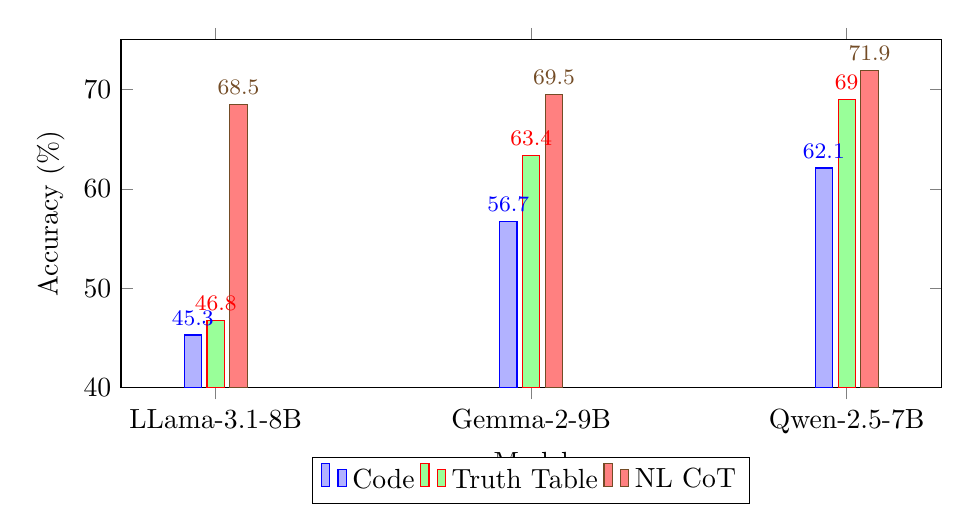
\begin{tikzpicture}
\begin{axis}[
    ybar,
    bar width=0.22cm,
    width=12cm,
    height=6cm,
    enlarge x limits=0.15,
    ylabel={Accuracy (\%)},
    xlabel={Model},
    symbolic x coords={LLama-3.1-8B, Gemma-2-9B, Qwen-2.5-7B},
    xtick=data,
    ymin=40,
    ymax=75,
    nodes near coords,
    legend style={at={(0.5,-0.2)},anchor=north,legend columns=3},
    every node near coord/.append style={font=\footnotesize},
]
\addplot+[style={fill=blue!30}] coordinates {(LLama-3.1-8B,45.3) (Gemma-2-9B,56.7) (Qwen-2.5-7B,62.1)};
\addplot+[style={fill=green!40}] coordinates {(LLama-3.1-8B,46.8) (Gemma-2-9B,63.4) (Qwen-2.5-7B,69.0)};
\addplot+[style={fill=red!50}] coordinates {(LLama-3.1-8B,68.5) (Gemma-2-9B,69.5) (Qwen-2.5-7B,71.9)};
\legend{Code, Truth Table, NL CoT}
\end{axis}
\end{tikzpicture}
\caption{Single-sample performance (\%) of three models on FOLIO across different reasoning modes.}
\label{fig:single_sample_bar}
\end{figure}